\section{Arbeitspakete}
Dieser Abschnitt beschreibt die Unterteilung des Projektes in Arbeitspakete und wie die Gruppenmitglieder die zugeteilten Arbeitspakte abarbeitet haben. Es wird auch auf den unvorhergesehenen Arbeitsbereitschaftsmangel der Gruppenmitglieder Herr Gregarek und Herr Dück eingegangen.

\subsection{Einteilung der Arbeitspakete}
Zunächst wurden die Arbeitspakete aus der Anforderungsanalyse abgeleitet. Aus dieser Ableitung sind folgende Arbeitspakete definiert worden:
\begin{enumerate}
	\item Entwicklung des grundlegenden Webseitendesigns für Desktop-Rechner
	\item Anpassung des Designs für mobile Geräte
	\item Entwicklung der Webseitennavigationsleiste
	\item Entwicklung der inhaltlichen Seiten des Webshops:
	\begin{itemize}
		\item Startseite
		\item Produktseite
		\item Rechtliche Seiten:
		\begin{itemize}
			\item[$\diamond$] Impressum
			\item[$\diamond$] Datenschutz
			\item[$\diamond$] AGB
		\end{itemize}
	\end{itemize}
	\item Entwicklung einer Schnittstellendatenbank zum Datenaustausch zwischen Webshop und SAP-System:
	\begin{itemize}
		\item Ansprechpartner der SAP-Gruppe für die Schnittstelle zum Webshop
		\item Entwurf von Tabellen für die Datenhaltung des Webshops 
	\end{itemize}
	\item Registrierungs- und Anmeldungsfenster designen und programmieren
	\begin{itemize}
		\item Möglichkeit den Kunden bieten die Anmeldeinformationen später verändern zu können
	\end{itemize}
	\item Entwickeln einer Suchfunktion:
	\begin{itemize}
		\item Autovervollständigung
		\item Erweiterte Suchfunktion, wo die Suche genauer eingegrenzt werden kann
		\item Auflistung der Suchergebnisse
	\end{itemize}
	\item Warenkorb
	\begin{itemize}
		\item Auflistung der Produkte, die sich im Warenkorb befinden
		\item Formular mit Mengenfeld, um ein Produkt in den Warenkorb zu packen
		\item Möglichkeit zur nachträglichen Änderung der Produkte im Warenkorb:
		\begin{itemize}
			\item[$\diamond$] Änderung der Bestellmenge
			\item[$\diamond$] Entfernen des Produkts aus dem Warenkorb
		\end{itemize}
	\end{itemize}
	\item Bestellvorgang:
	\begin{itemize}
		\item Bestellroutine mit folgenden Schritten:
		\begin{itemize}
			\item[$\diamond$] Wahl der Versandart
			\item[$\diamond$] Nachträglichen Änderung der Bestellmenge der Produkte
			\item[$\diamond$] Wahl Zahlungsart
			\item[$\diamond$] Wahl Lieferadresse
			\item[$\diamond$] Bestellübersichtseite zur Kontrolle vor den Absenden der Bestellung
		\end{itemize}
		\item Einsicht des aktuellen Status der Bestellung
		\item Möglichkeit die Bestellung zu stornieren
	\end{itemize}
	
	\item Erstellung eines Marketing Mix
	\item Bewertungsfunktion von Artikel (mit Kommentarfunktion)
	\item Email-Versand
	\begin{itemize}
		\item Klasse für den Email-Versand entwerfen
		\item Designen der Bestätigungs-Emails
	\end{itemize}					 
\end{enumerate}

Die oben genannten Arbeitspakete hat sich die Gruppe untereinander aufgeteilt. Stefan Schnürer hat Arbeitspakete 1,3 und 4 übernommen. Benedikt Brüntrup übernahm die Arbeitspakete 5, 6 und 7. Michael Dück hatte sich bereit erklärt die Arbeitspakte 2, 11 und 12 zu bearbeiten. Raphael wollte die Arbeitspakete 8, 9 und 10 abarbeiten.


%Nachfolgend soll auf die einzelnen Zwischenschritte des Projektes eingegangen werden.Das Projekt beginnt mit der Projektplanung. Hierbei werden die Arbeitspakete definiert und an den entsprechenden Gruppenmitgliedern verteilt. Pro Arbeitspaket wird eine Bearbeitungsdauer von zwei Wochen festgelegt. Es wird ein Projektzeitplan sowie eine Risikoanalyse erstellt. Im Anschluss daran werden grobe Design Entwürfe für die Homepage erstellt. Es wird sich für den Design Entwurf von Herrn Brüntrup entschieden. Die Homepage wird in einem matten Grün-Ton designt, um den Kunden die Umweltaspekte von Fahrrädern zu verdeutlichen.
%\textbf{Was machen Herr Gregarek und Herr Dück?}

\subsection{Arbeitspaket von Herrn Schnürer}

In den nachfolgenden Wochen wird die Homepage nach Vorlage des Designs Entwurfs von Herrn Brüntrup erstellt. Der erste Prototyp der Seite basiert auf den Standardaufbau einer Webseite. Dabei wird der Inhalt der Seite in HTML geschrieben, während eine CSS Datei für das Seitenlayout der Webseite verantwortlich ist. \textit{Abbildung 5} zeigt einen ersten groben Designentwurf der Startseite:



\begin{figure}[H]
\begin{center}
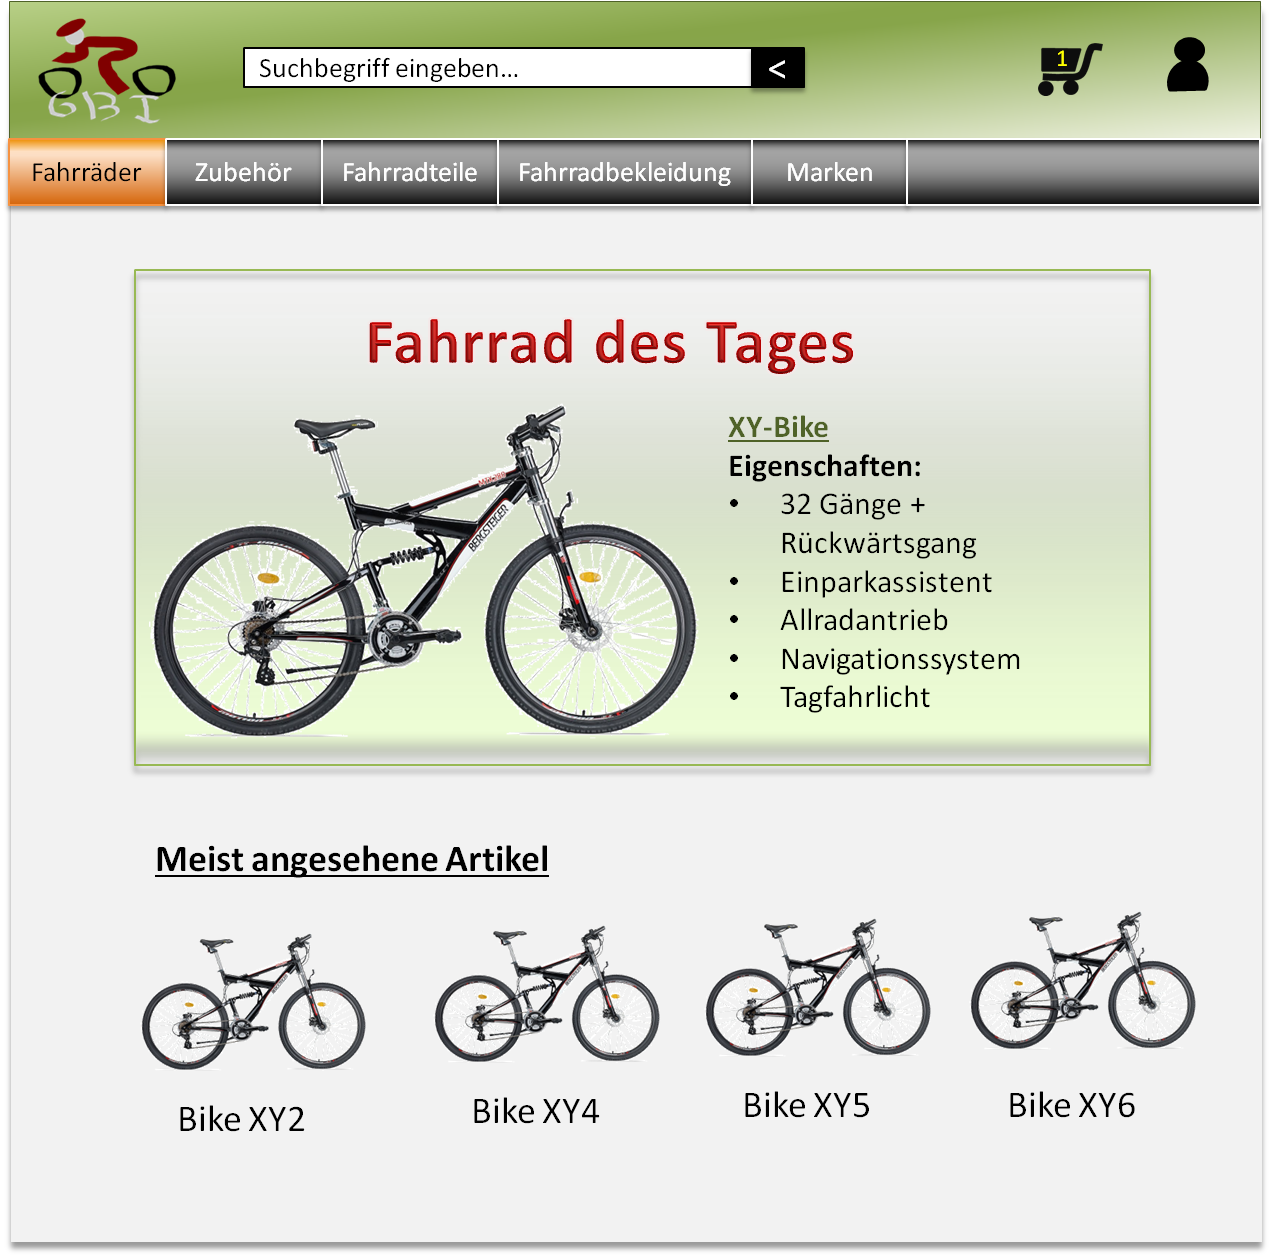
\includegraphics[width=150mm]{Bilder/Abbildung2-GroberDesignEntwurfDesWebshops.png}
\end{center}
\caption{Erster grober Designentwurf der Startseite}
\end{figure}



Die Startseite wird zunächst mit zwei einfachen Artikeln versehen. Sie sollen eine grobe Vorstellung liefern, wie die fertige Startseite aussehen könnte.
In den darauf folgenden Wochen liegt der Fokus auf die Seitennavigation in der Kopfzeile (nachfolgend Header) der Seite. Die Seitennavigation wird mithilfe von CSS an den Designentwurf angepasst. Es werden die Hauptkategorien „Fahrräder“, „Zubehör“, „Fahrradteile“, „Fahrradbekleidung“, „Marken“ und eine Rubrik „HowTo“ angezeigt. Letztere verlinkt auf eine Internetquelle, mit dessen Hilfe die Seitennavigation umgesetzt wurde. Diese Kategorie dient den anderen Gruppenmitgliedern als Referenz und wird in späteren Versionen des Webshops wieder entfernt. Fährt der Nutzer mit der Maus über die Kategorie „Fahrräder“ öffnet sich ein Drop-Down-Menü, welches den Nutzer verschiedene Fahrradmodelle auswählen lässt. Die komplette Seitennavigation wurde in CSS3 umgesetzt. CSS3 kann von nahezu jeden aktuellen Browser gelesen werden und bietet zudem den Vorteil, dass der entsprechende Code in der bisherigen CSS-Datei eingefügt werden kann. Da CSS3 unabhängig von Java Script ist, lässt sich die Seite zudem problemlos bedienen, wenn Java Script auf den jeweiligen Browsern deaktiviert ist. Dies begründet die Entscheidung CSS3 für die Seitennavigation zu verwenden.
\textit{Abbildung 6} und \textit{7} zeigen den bisherigen Seitenprototypen:



\begin{figure}[H]
\begin{center}
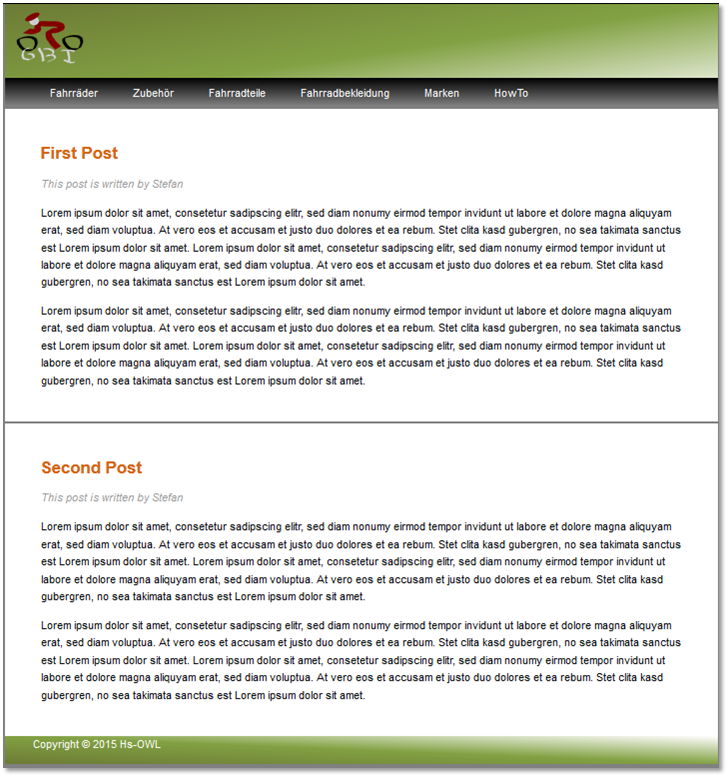
\includegraphics[width=150mm]{Bilder/Abbildung3-Seitenprototyp.png}
\end{center}
\caption{Seitenprototyp}
\end{figure}


\begin{figure}[H]
\begin{center}
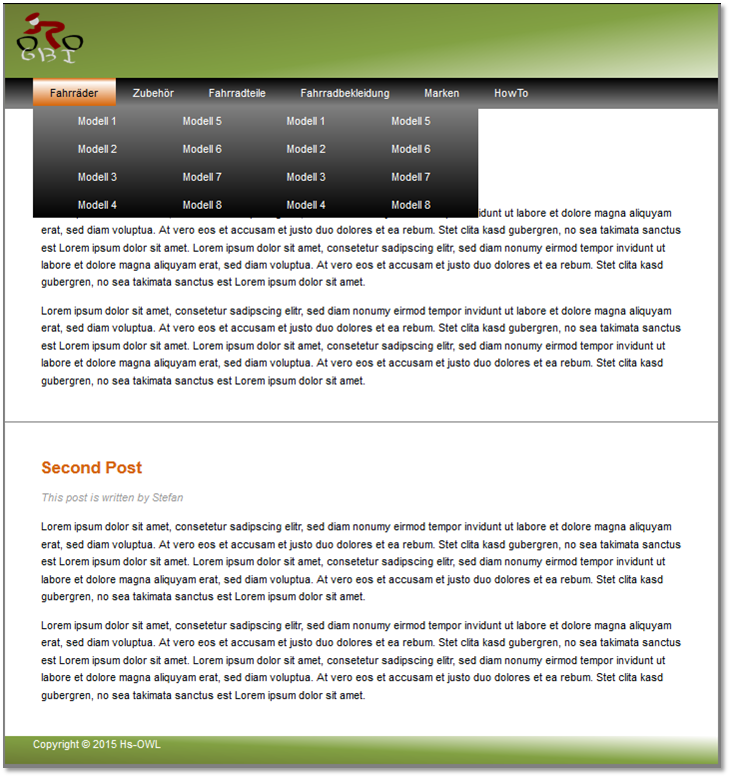
\includegraphics[width=150mm]{Bilder/Abbildung4-SeitenprototypMitDropDownMenue.png}
\end{center}
\caption{Seitenprototyp mit Drop-Down-Menü}
\end{figure}



%Ein paar Wochen später wird sich dazu entschlossen das Programm „Eclipse“ zum Programmieren des Webshops zu nutzen. Das Programm bietet neben einer Autovervollständigung und der Unterstützung mehrerer Programmiersprachen noch zusätzlich den Vorteil, dass es durch Plug-Ins erweiterbar ist. So lässt sich „Eclipse“ durch das Plug-In „GitHub“ erweitern. „GitHub“ ist eine Cloud basierte Lösung zum gemeinsam bearbeiten von Programmcode. Das komplette Projekt wird dabei auf einen Server hochgeladen. Jedes Gruppenmitglied, das einen Acount bei „GitHub“ erstellt hat, kann dem Projekt beitreten, indem es bei den Gruppen- Administrator um Erlaubnis bittet. Dadurch kann ein Dokument von mehreren Gruppenmitgliedern gemeinsam bearbeitet werden. So entstehen mehrere Versionen von einem Dokument, die anschließend wieder zu einem Dokument zusammengefügt werden können.%
Im Laufe der nächsten Woche wird die Startseite des Webshops gemäß dem Designentwurfs erstellt (siehe \textit{Abbildung 8}). Auf der Startseite ist das „Angebot des Tages“ zu sehen. Es gibt eine Kurzbeschreibung zu dem Artikel mit den wichtigsten Eigenschafen. Der untere Teil der Startseite zeigt die meist angesehenen Artikel des Nutzers an. 

\begin{figure}[H]
\begin{center}

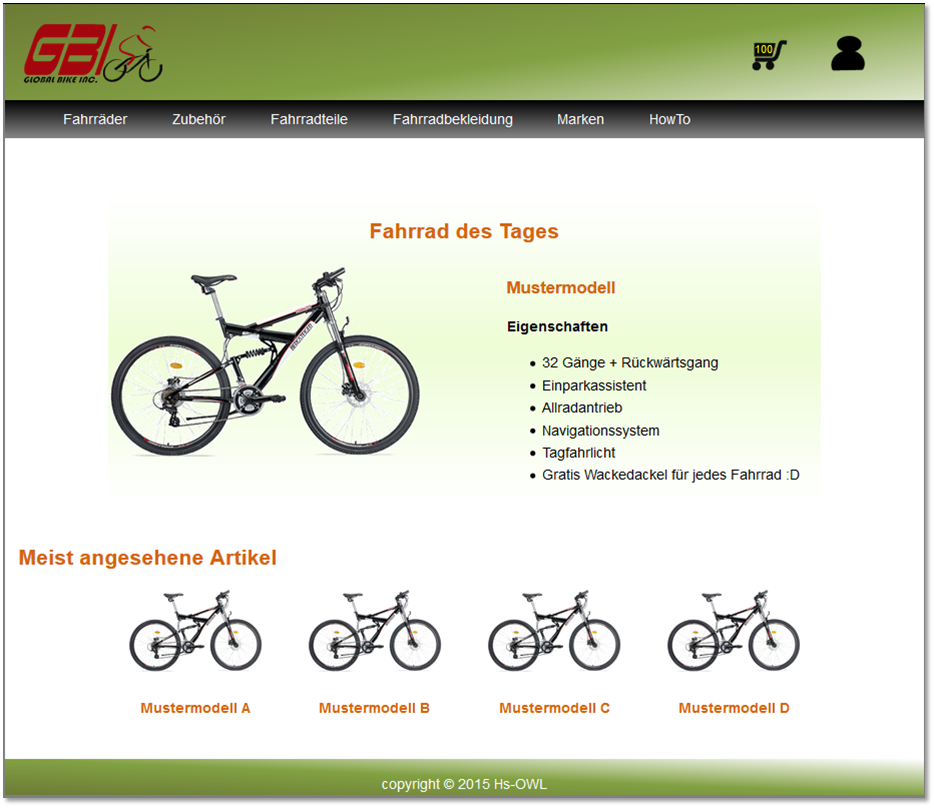
\includegraphics[width=150mm]{Bilder/Abbildung5-StartseiteDesWebshops.PNG}
\end{center}
\caption{Startseite des Webshops}
\end{figure}

In den nächsten Tagen wird das Thema Rechtschutz behandelt. Dem Webshop werden ein Impressum, die AGB sowie Hinweise zum Datenschutz hinzugefügt:

\begin{figure}[H]
\begin{center}
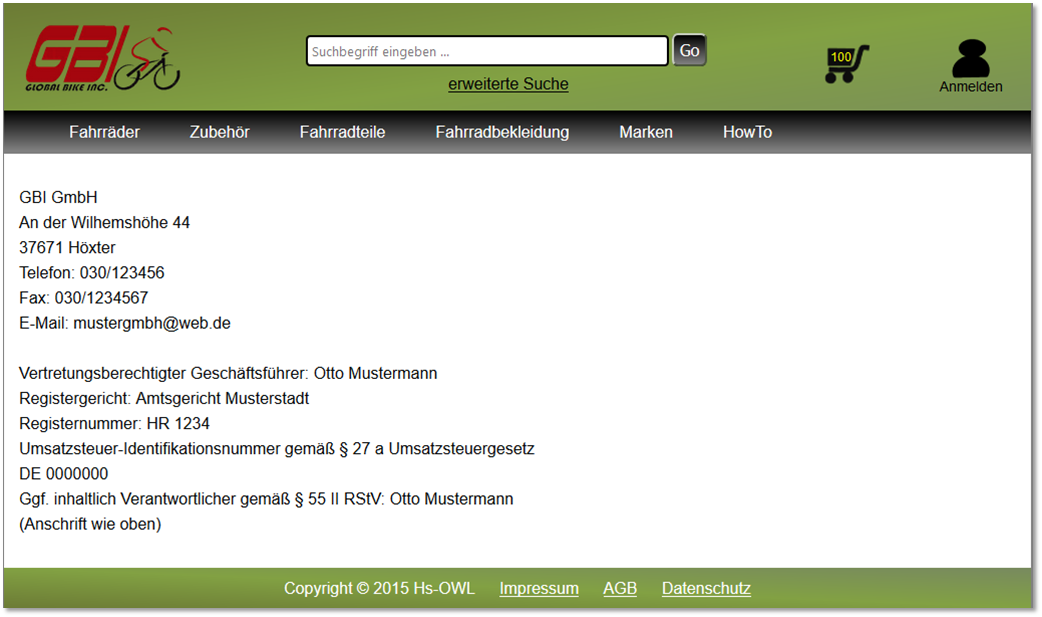
\includegraphics[width=150mm]{Bilder/Abbildung6-ImpressumDesWebshops.PNG}
\end{center}
\caption{Impressum des Webshops}
\end{figure}

\begin{figure}[H]
\begin{center}
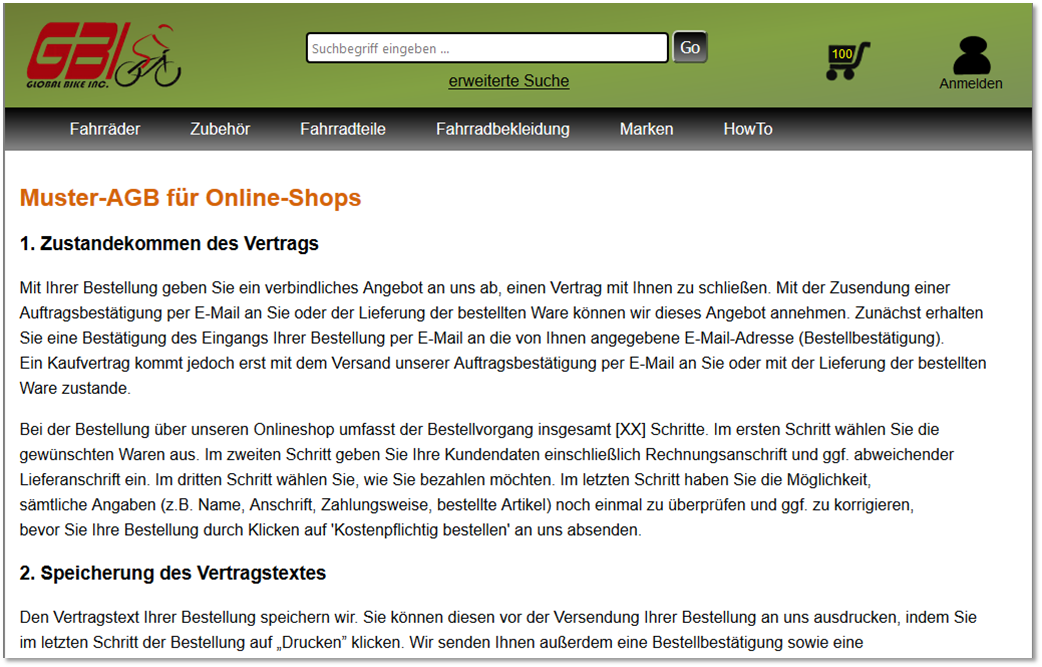
\includegraphics[width=150mm]{Bilder/Abbildung7-AGBDesWebshops.PNG}
\end{center}
\caption{AGB des Webshops}
\end{figure}

\begin{figure}[H]
\begin{center}
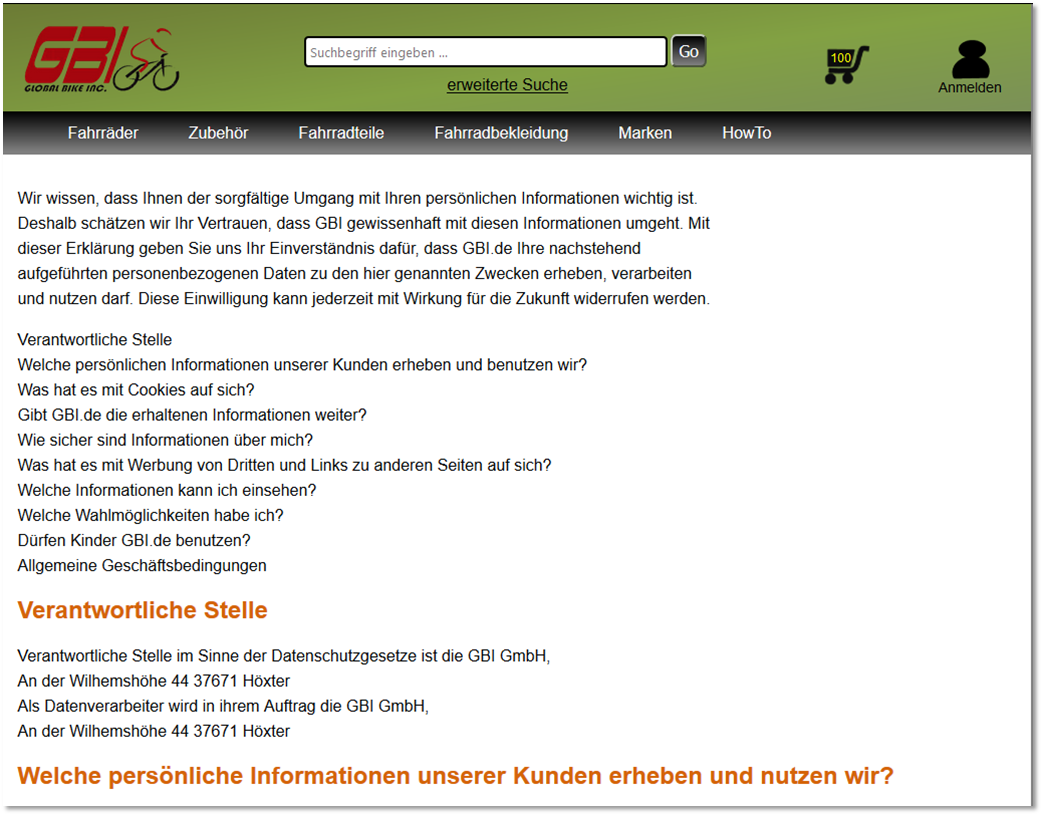
\includegraphics[width=150mm]{Bilder/Abbildung8-DatenschutzDesWebshops.PNG}
\end{center}
\caption{Datenschutz des Webshops}
\end{figure}

\subsection{Arbeitspakete von Herrn Brüntrup}
In diesem Abschnitt wird beschrieben, wie Herr Brüntrup seine Arbeitspakete gelöst hat. Zudem wird in diesem Abschnitt noch beschrieben welche Arbeitspakete wegen Zeitmangel und fehlender Arbeitsbereitschaft zusätzlich noch übernommen wurden.

\subsubsection{Arbeitspaket 5: Die Schnittstellendatenbank}
Die Datenbank stellt die Schnittstelle zwischen dem SAP-System und dem Webshop da. Aus diesem Grund wurde die Datenbankstruktur in der ersten Woche nach der Arbeitspaketverteilung zusammen mit Mitgliedern der SAP-Gruppe entworfen.\\

\textbf{Gründe für die Schnittstellendatenbank}\\
Die Gründe warum die Kommunikation mit einer Schnittstellendatenbank gelöst wurde, wird in den folgenden Sätzen genannt. Der erste Grund war die Verfügbarkeit. Der Webshop sollte auch erreichbar sein, wenn mal keine Verbindung zum SAP-System besteht. Der SAP-Server steht extern bei einer Hochschule in Magdeburg. Es könnte also schon mal dazu kommen, dass das System nicht erreichbar ist. Ein anderer Grund war die Flexibilität. Die Datenhaltung sollte flexibel erweiterbar sein. Soll die Webseite z.B. durch eine 360$^\circ$-Ansicht des Fahrrads erweitert werden, können einfach die benötigten Felder zur Datenbank hinzugefügt werden. Beim SAP-System ist das nur beschränkt möglich. Der Zugriff auf das SAP-System wird mit vordefinierten Funktionen gelöst. Diese Funktionen werden \glqq Business Application Programming Interface (BAPI)\grqq{} genannt. Da die SAP-Gruppe beim SAP-System keine Berechtigungen hat neue BAPIs zu erstellen, wäre somit die Erweiterbarkeit des Webshops sehr eingeschränkt.\\

\textbf{Aufbau der Schnittstellendatenbank}\\
Nun wird der zu Beginn geplante Aufbau der Schnittstellendatenbank erläutert. Die zu Beginn geplante Datenbank bestand aus den Relationen \glqq Kunde\grqq{}, \glqq Bestellungen\grqq{}, \glqq Produkte\grqq{} und \glqq Produktbilder\grqq{}. Die Relation \glqq Kunde\grqq{} enthält die Login-Daten des Kunden sowie dessen Adresse. Die Relation \glqq Bestellungen\grqq{} enthält alle Angaben zur Bestellung. Angaben sind z.B. die Zahlungs- und Versandart sowie der Status der Bestellung. Die vorletzte genannte Relation beinhaltet alle Angaben zu den Produkten, die beim Webshop verkauft werden sollen. Ihr wurde deswegen auch der Name \glqq Produkte\grqq{} gegeben. Die Relation \glqq Produktbilder\grqq{} enthält Pfadangaben, wo auf den Server die Produktbilder abgelegt sind. Da zu einen Produkt mehrere Produktbilder abgelegt werden können, wurde sich auf eine extra Tabelle für die Produktbilder geeinigt.

Eine Relation, die die Produkte einer Bestellung enthält, wurde zunächst vergessen umzusetzen. Das Vergessen der Relation fiel erst auf, als die SAP-Gruppe mit der Umsetzung des Bestellvorgangs bei der SAP-Schnittstelle beginnen wollte. Zur Lösung des Problems fügte die SAP-Gruppe nun nachträglich eine Relation \glqq Bestellprodukte\grqq{} zur Datenbank hinzu. Diese Relation steht in Beziehung mit den Relationen \glqq Bestellungen\grqq{} und \glqq Produkte\grqq{}.

Als Datenbank-Server wurde sich auf MYSQL geeinigt. Dieser Server lässt sich problemlos auf Linux installieren. Es war wichtig, dass die Datenbank unter Linux läuft, da die Server-Gruppe einen Linux-Server aufsetzen wollte. Zudem bietet MYSQL den Vorteil, dass auf eine MYSQL-Datenbank mit der Programmiersprache PHP gut zugegriffen werden kann. Die SAP-Gruppe wollte die Datenbank mit einer selbst geschriebenen JAVA-Anwendung füllen. Auch von JAVA aus kann gut auf eine MYSQL-Datenbank zugegriffen werden. Ein weiterer Grund für die Nutzung der MYSQL-Datenbank war, dass die Softwaresammlung XAMPP einen MYSQL-Server beinhaltet. Die Softwaresammlung XAMPP wurde von der Webshop-Gruppe als Testserver zum Testen der Webseite auf den Hochschulrechnern verwendet. \\
Die \textit{Abbildung 12} zeigt das \glqq Entity-Relationship-Diagramm (ERD)\grqq{}. Dieses Diagramm ist die erste Version der Datenbank, die zusammen mit der SAP-Gruppe entworfen wurde. 

\begin{figure}[H]
	\begin{center}
		\fbox{
			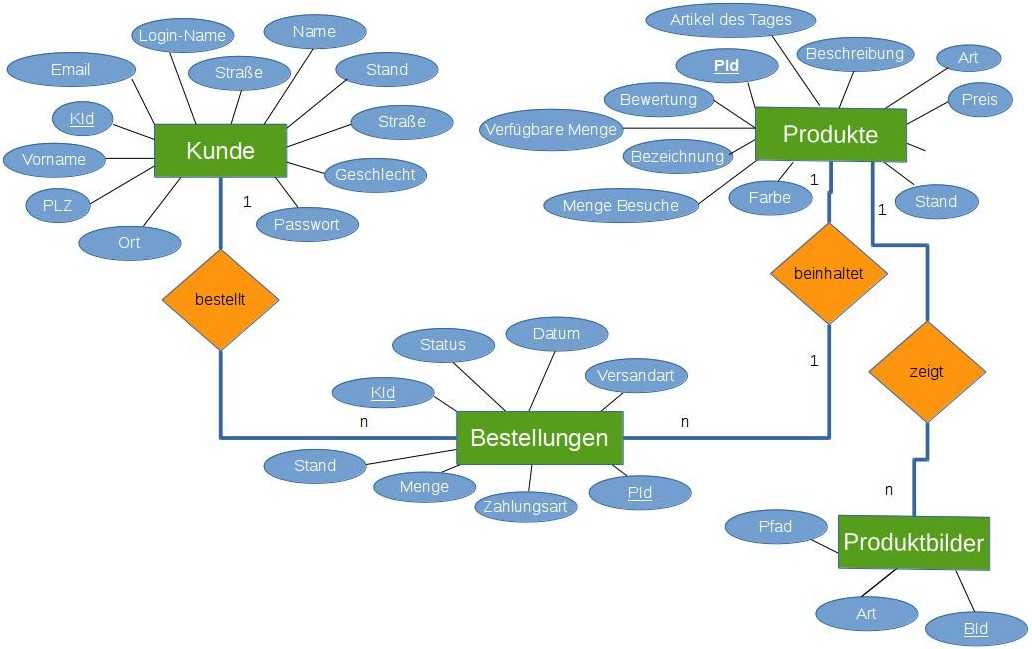
\includegraphics[width=150mm]{Bilder/Abbildung10-erd_alt.jpg}
		}
	\end{center}
	\caption{Erster Datenbankentwurf}
\end{figure}

Da es ursprünglich bemängelt wurde, dass das Projekt noch nicht den für das Modul benötigten Zeitaufwand aufweisen wurde, wurde beschlossen das Arbeitspaket \glqq Bewertung\grqq{} mit einer Kommentarfunktion zu erweitern. Somit sollte der Kunde auch ein Kommentar für seine Bewertung äußern können. Dafür musste die Datenbank etwas angepasst werden. Vorher war einfach ein Attribut \glqq Bewertung\grqq{} in der Relation \glqq Produkte\grqq{} vorzufinden. Um die Kommentare für die Bewertung speichern zu können, wurde die Datenbank um eine Relation \glqq Kommentare\grqq{} erweitert. Diese Relation beinhaltet ein Datenfeld, wo die Bewertung des Kunden (von 1-5 Sterne) gespeichert wird. Ein weiteres Datenfeld der Relation enthält den Bewertungstext. \\
Als mit der Suchfunktion und der Navigation begonnen wurde, fiel schnell auf, dass benötigte Attribute und Tabellen für die Navigation vergessen wurden. Somit wurde eine neue Relation \glqq Produktkategorie\grqq{} zur Datenbank hinzugefügt. Diese Relation steht mit der Relation \glqq Produkte\grqq{} in Beziehung und beinhaltet alle Produktkategorien, die der Webshop anbieten soll. Unter Produktkategorien wird beim Webshop die Festlegung verstanden, ob das Produkt ein Ersatzteil, ein Fahrrad, Zubehör usw. ist. Eine zweite Relation, die mit der Relation Produkte in Beziehung steht, ist die Relation \glqq Bauart\grqq{}. Dieses Relation wird nur verwendet, wenn das Produkt ein Fahrrad ist. In dieser Relation sind alle beim Webshop angebotenen Bauarten aufgelistet. Unter Bauart wird bei diesen Webshop verstanden, ob es sich um ein Mountainbike, Trekkingbike usw. handelt.

Die \textit{Abbildung 13} zeigt die endgültige Struktur der Schnittstellendatenbank mit allen nachträglich hinzugefügten Relationen. 
\begin{figure}[H]
	\begin{center}
		\fbox{
			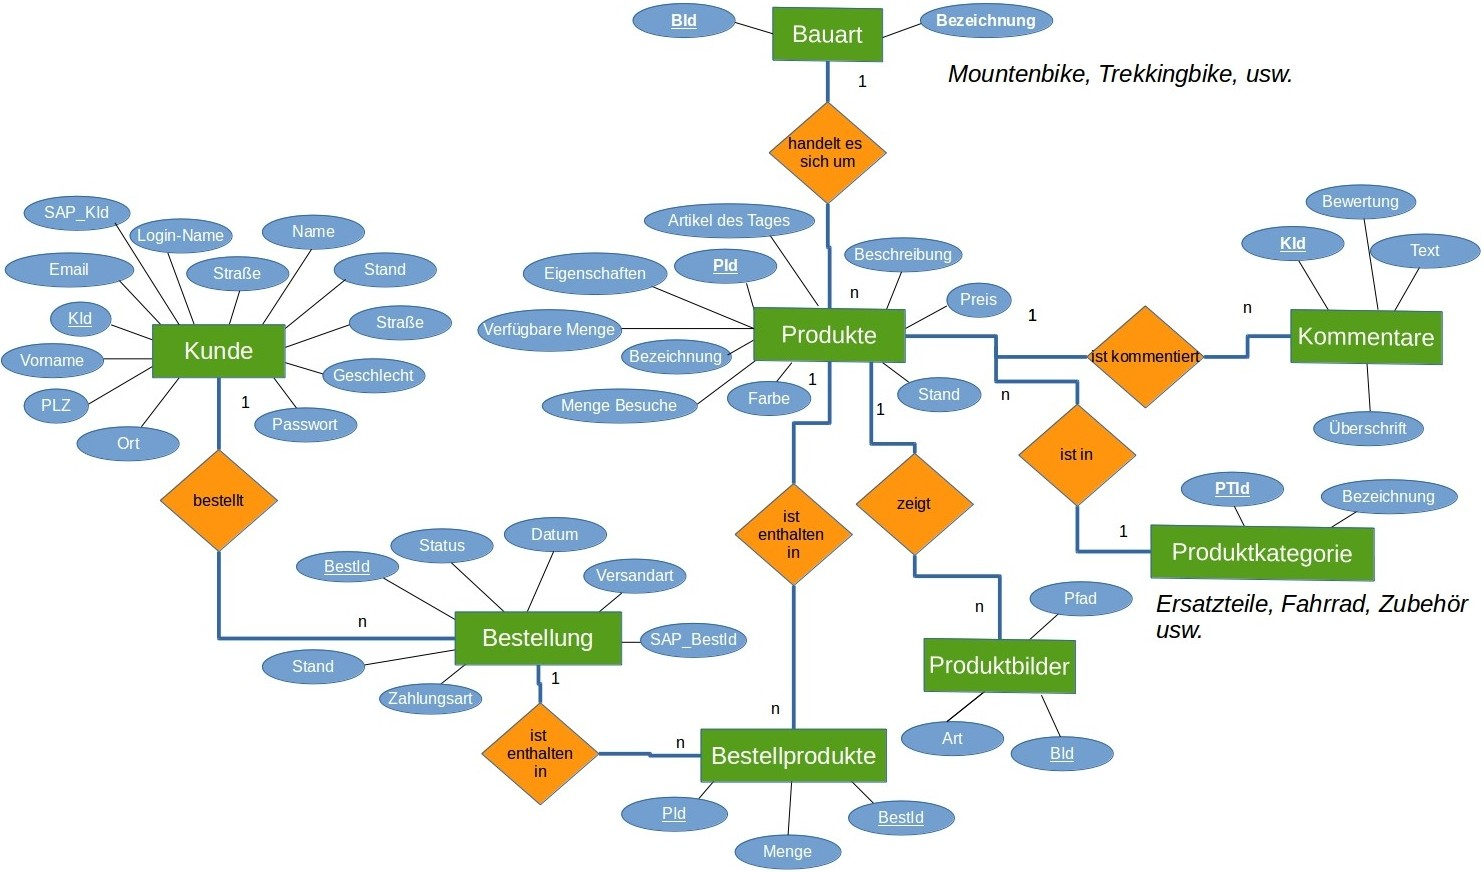
\includegraphics[width=150mm]{Bilder/Abbildung11-erd.jpg}
		}
	\end{center}
	\caption{Endgültiger Datenbankentwurf}
\end{figure}

\textbf{Wahl der PHP-API zum Datenbankzugriff}\\
Um von PHP aus auf eine MYSQL-Datenbank zugreifen zu können, gibt es mehrere Möglichkeiten. In dieser Ausarbeitung werden die Zugriffsmöglichkeiten kurz verglichen und dann erläutert, welche davon für das Projekt benutzt wurde.

Die erste Möglichkeit ist die PHP-API \glqq ext/mysql \grqq{}. Diese API ist veraltet und wird nicht mehr weiterentwickelt. Sie unterstützt noch nicht alle MYSQL 5.1+ Funktionalitäten und ist stellenweise mit neuen PHP-Versionen nicht mehr nutzbar. Diese Erweiterung nutzt den prozeduralen Ansatz. Die nächste Möglichkeit ist die PHP-API \glqq PDO\grqq{}. Diese API unterstützt fast alle Funktionalitäten von MYSQL 5.1+. Sie bietet zudem den Vorteil, dass die API auch zum Zugriff auf andere SQL-basierten Datenbanken genutzt werden kann. Diese API hat einen objektorientierten Aufbau.  Die letzte Zugriffsmöglichkeit bietet die API \glqq ext/mysqli\grqq{}. Sie unterstützt alle MYSQL 5.1+ Funktionalitäten und kann objektorientiert und prozedural programmiert werden.

Die Auswahl fiel auf die API \glqq ext/mysqli\grqq{}. Die Gründe hierfür waren, dass die API alle Funktionalitäten der neusten MYSQL-Version unterstützt, regelmäßig auf die neuesten MYSQL-Funktionen angepasst wird und schon Quellcodes von alten Projekten übernommen werden konnte. Die \textit{Abbildung 14} zeigt die Eigenschaften der drei APIs nochmal in einer Tabelle zusammen gefasst.
\begin{figure}[H]
	\begin{center}
		\fbox{
			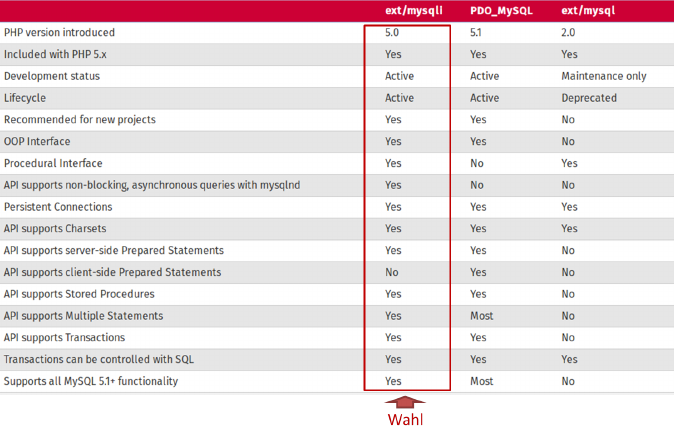
\includegraphics[width=150mm]{Bilder/Abbildung12-mysql_apis.png}
		}
	\end{center}
	\caption{Überblick der PHP-APIs zum Datenbankzugriff}
\end{figure}

\textbf{Die Konfigurationsdatei}\\
Um auf eine MYSQL-Datenbank zugreifen zu können, werden üblicherweise mehrere Zugangsdaten benötigt. Die Zugangsdaten, die mindestens benötigt werden, sind der Datenbankbenutzername, das Passwort zum Benutzername, der Datenbankname und die IP-Adresse des Servers. Damit diese Zugangsdaten nicht bei jeden Datenbankzugriff im Quelltext angegeben werden müssen, wurden diese Angaben in eine Konfigurationsdatei ausgelagert. Wird die Webseiten später mal auf einen anderen Webserver betrieben, so müssen die Datenbankzugangsdaten nur in dieser Datei geändert werden. Die Konfigurationsdatei ist extra gesichert worden, damit sie nicht direkt im Browser geöffnet werden kann. Der Datei wurde als Dateiendung \glqq *.php.inc\grqq{} angehangen. Mit einer bestimmten Zeile in einer Konfigurationsdatei für den Webserver wurde das Öffnen von \glqq *.inc\grqq{}-Dateien den Browser untersagt. Die Konfigurationsdatei trägt den Namen \glqq .htaccess\grqq{} und befindet sich im Home-Vezeichnis der Webseite. Mehr zur \glqq .htaccess\grqq{}-Datei kann im Abschnitt \glqq Webshopsicherheit\grqq{} gelesen werden.

Der \textit{Quellcode 1} zeigt die Konfigurationsdatei des Webshops. In dieser Datei sind die benötigten Datenbankzugangsdaten und die festgelegte Email-Adresse zu lesen, von der alle Bestätigungs-Emails versendet werden sollen. Zudem sind in der Konfigurationsdatei die Bankdaten definiert, die dem Kunden mitgeteilt werden, wenn er als Zahlungsart \glqq Vorkasse\grqq{} ausgewählt hat.

\newpage
\begin{center}
	\begin{lstinputlisting}[language=PHP, caption={Die Konfigurationsdatei}]
		{Quellcode/config.php.inc}
	\end{lstinputlisting}
\end{center}

\textbf{Die Datenbankzugriffsklasse}\\
Beim Webshop wird nicht direkt über die \glqq MYSQLi\grqq{}-API auf die MYSQL-Datenbank zugegriffen. Es wurde für den Datenbankzugriff extra eine Klasse entwickelt, die als Schnittstelle zwischen den Webshop und der \glqq MYSQLi\grqq{}-API fundiert. Diese Klasse bestand schon von alten Projekten und wurde aus folgendem Grund entwickelt. Sie wurde entwickelt, damit nur an einer Stelle das Projekt verändert werden muss, wenn zu einen späteren Zeitpunkt mal ein anderes API verwendet werden soll. Dieses ist z.B. der Fall, wenn zu eine andere Datenbank verwendet werden soll.

\newpage
\subsubsection{Arbeitspaket 6: Registrierungs- und Anmeldungsfenster designen und programmieren}
Dieser Abschnitt beschreibt, wie beim Webshop die Registrierung und Anmeldung umgesetzt wurde. Zudem wird die Umsetzung einer Funktion des Webshops beschrieben, wo der Kunde seine Profildaten ändern kann.\\

\textbf{Der Registrierungsvorgang}\\
Auf dieser Webseite läuft die Registrierung wie in den folgenden Sätzen beschrieben ab. Zunächst tippt der Neukunde die von der Webseite verlangten persönlichen Informationen in ein Formular ein und bestätigt die Eingabe durch einen Klick auf den Bestätigungsbutton. Wenn beim Webbrowser des Neukunden JavaScript nicht deaktiviert ist, überprüft der Webbrowser mit einem JavaScript die Eingabe bevor sie zum Webserver weitergeleitet wird. Die Eingabe wird nur weitergeleitet, wenn diese vom JavaScript aus als gültig anerkannt wurde. Bei ungültiger Eingabe wird auf der Webseite eine Fehlermeldung ausgegeben. Der JavaScript ist keine endgültige Eingabeüberprüfung, dieser dient nur dafür unnötigen Datenverkehr zu minimieren. JavaScript besitzt den Nachteil, dass dieser beim Webbrowser deaktiviert werden kann. Bei deaktivierten JavaScript wird somit die Eingabe unüberprüft an den Webserver weitergeleitet. Somit muss die Eingabe nochmal beim Webserver auf Gültigkeit überprüft werden.  Der Neukunde wird also erst in die Kunden-Tabelle der Datenbank geschrieben, wenn die serverseitig programmierten Überprüffunktionen die Eingabe als gültig angesehen haben. Wurde die Eingabe als ungültig anerkannt, so wird auch bei der serverseitigen Programmierung eine Fehlermeldung auf der Webseite angezeigt. Nachdem der Kunde erfolgreich in der Kundendatenbank angelegt wurde, bekommt der Neukunde eine Bestätigungsmail zu gesendet. Der Neukunde kann sich erst erfolgreich am System anmelden, wenn dieser den in der Email enthaltenden Link ausgeführt hat. 

Das Passwort des Kunden wird nicht in Klartext in die Datenbank gespeichert. Bevor es in die Datenbank geschrieben wird, wird das Passwort mit einen \glqq MD5-Hash-Algorithmus\grqq{} unkenntlich gemacht. Der MD5-Hashwert ist nicht mit einen Schlüssel wieder invertierbar. Er kann zur Speicherung von Passwörtern verwendet werden, da beim \glqq MD5-Hash-Algorithmus\grqq{} der gleiche Input immer den gleichen Output erzeugt. Somit wird beim Login-Check einfach auch das eingegebene Passwort unkenntlich gemacht und verglichen, ob es mit den Wert in der Datenbank übereinstimmt.\\ Die \textit{Abbildung 15} zeigt den Registrierungsvorgang nochmal als BPMN dargestellt.\\

\begin{figure}[H]
	\begin{center}
			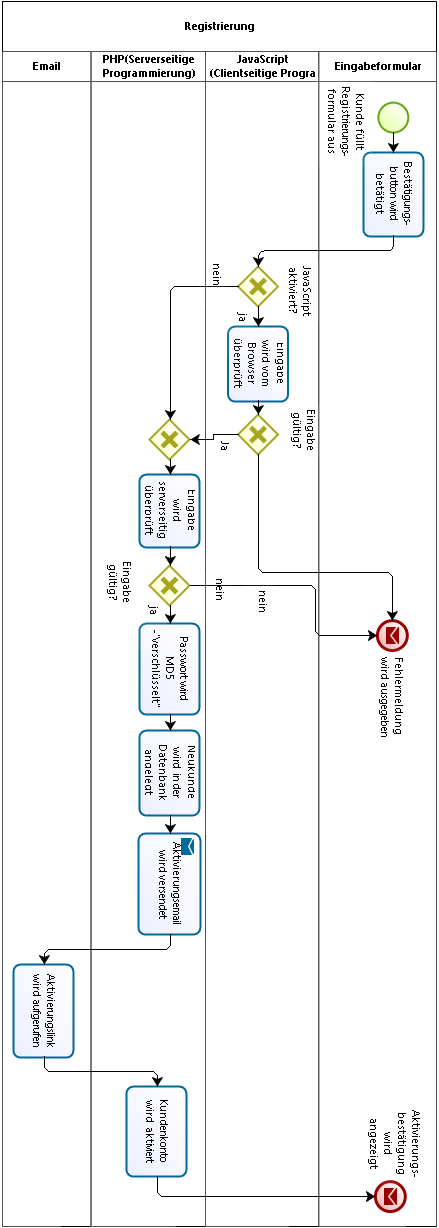
\includegraphics[width=225pt]{Bilder/Abbildung13_Reg_Vorgang.png}
	\end{center}
	\caption{Der Registrierungsvorgang}
	\label{fig:Abbildung 13}
\end{figure}


\textbf{Der Anmeldungsvorgang}\\
Der Anmeldungsvorgang läuft ähnlich wie der Registrierungsvorgang ab. Der Kunde tippt als Benutzernamen seine Email-Adresse und als Passwort das bei der Registrierung angegebene Passwort in das Anmeldeformular ein. Wie bei der Registrierung überprüft ein JavaScript die Eingabe bevor diese an den Server weitergeleitet wird. Die vorherige Überprüfung ist wieder nur bei aktivierten JavaScript im Webbrowser möglich. Deswegen wird die Überprüfung bei der Anmeldung auch nochmal vom Server überprüft. Hat der Kunde eine gültige Eingabe getätigt, so wird die Email-Adresse und das Passwort mit den Datensätzen in der Kunden-Tabelle der Datenbank verglichen. Um den Vergleich ausführen zu können wird bei der Anmeldung auch das Passwort durch den  \glqq MD5-Hash-Algorithmus\grqq{} unkenntlich gemacht. Wurde in der Tabelle ein Datensatz gefunden, wo Email-Adresse und Passwort übereinstimmen, so wird der Kunde eingeloggt. Wurde keine Übereinstimmung gefunden, so wird auf der Webseite eine Fehlermeldung ausgegeben.\\ 
Der Einlogvorgang wurde wie folgt umgesetzt. Die Anmelde-Email-Adresse wird in einer SESSION-Variable gespeichert. Der SESSION-Variable wurde der Name \glqq \$\_SESSION['angemeldet']\grqq{} gegeben. An Hand dieser Variable erkennt der Webshop, ob der Kunde angemeldet ist oder nicht. Wurde die Variable angelegt und enthält einen Wert, so wird dieses als angemeldet interpretiert. Die Abmeldung erfolgt einfach durch das Löschen dieser Variable. Eine SESSION-Variable behält die enthaltenden Daten über mehrere Seitenaufrufe. Wenn nicht mehr auf die Variable zugegriffen wird, werden die Daten dieser Variable automatisch nach einer bestimmten Zeit gelöscht. Ob der Kunde angemeldet ist, muss in einer SESSION-Variable zwischengespeichert werden, da das HTTP-Protokoll verbindungslos ist. Es wird also jede HTTP-Anfrage isoliert betrachtet. Ohne die SESSION-Variable könnte sich somit der Webserver nicht merken, dass der Kunde angemeldet ist. Einer Session wird in PHP eine eindeutige \glqq SESSION-ID\grqq{} zugeordnet. Diese SESSION-ID wird entweder als Cookie im Browser abgespeichert oder immer der Seiten-URL mit übergeben. Wird die SESSION-ID in einem Cookie im Browser abgespeichert, so wird dieser beim Schließen des Browsers gelöscht. Die Daten, die in der SESSION-Variable abgespeichert sind, werden auf der Serverseite zwischengespeichert und nicht im Browser. Die SESSION-ID wird von Browser bei jeder Anfrage an den Server weitergeleitet. An Hand dieser SESSION-ID kann der Server die SESSION-Variable zu den entsprechenden Browser zuordnen.\\

\textbf{Die clientseitige Überprüfung}\\
Wenn JavaScript aktiviert ist, werden, wie oben schon erwähnt, die Formulareingaben zuvor im Browser überprüft. Dafür wird beim Formular den Attribut \glqq onsubmit\grqq{} eine JavaScript-Funktion übergeben. Die Formulareingabe wird hierbei nur an den Server weitergeleitet, wenn diese Methode als Rückgabewert \glqq true\grqq{} zurückgibt. Die JavaScript-Funktion überprüft bei der Eingabe, ob überhaupt ein Text in die Textfelder eingegeben wurde und die Eingabe gültig ist. Zum Beispiel darf eine Postleitzahl nur aus 5 Ziffern bestehen. Die clientseitige Programmierung findet bei der Anmeldung in der Datei \glqq /Funktions/JS/anmeldung.js\grqq{} und bei der Registierung in der Datei \glqq /Funktions/JS/registrierung.js\grqq{} statt.

Der \textit{Quellcode 2} zeigt in vereinfachter Version das Login-Formular. Beim \glqq form\grqq{}-Tag kann das \glqq onsubmit\grqq{}-Attribut gefunden werden. Dieses Attribut startet beim Klick auf den Submit-Button die enthaltende JavaScript-Funktion. Das Attribut lässt nur die Durchführung des Submits zu, wenn die JavaScript-Funktion als Rückgabewert den Wert \glqq true\grqq{} zurückliefert.

Um unnötigen Quelltext zu umgehen, wurde ein Teil des Eingabeüberprüfungsquellcode in eine andere JavaScript-Datei ausgelagert. Der ausgelagerte Quellcode wird bei jeden Formular benötigt. Dieser Quellcode überprüft, ob alle Pflichtfelder ausgefüllt sind. Die ausgelagerte Funktion trägt den Namen \glqq sindAlleFelderAusgefuellt\grqq{} und befindet sich in der Datei \glqq /Funktions/JS/vorcheck\_std\_funktionen.js\grqq{}. Der Funktion werden beim Aufruf drei Parameter übergeben. Der erste Parameter erhält ein Array. Dieses Array enthält die Feldnamen der Textfelder, wovon die Eingabe überprüft werden soll. Der zweite Parameter enthält wiederum ein Array. Dieses Array enthält die Meldungswörter, die in der Fehlermeldung für das jeweilige Textfeld eingesetzt werden sollen. Die Meldungswörter werden in die Fehlermeldung eingesetzt, wenn das Textfeld nicht gefüllt ist. Beim letzten Parameter wird der Name des Formulars angeben, worauf sich die Textfelder befinden. Sind nicht alle Felder ausgefüllt, erstellt die Funktion eine Fehlermeldung und gibt diese als Rückgabewert aus.\\
In die Auslagerungsdatei wurden zudem Funktionen zur Überprüfung der Email-Adresse oder ob die Eingabe eine Zahl ist abgelegt. Die Funktionen in den Dateien \glqq /Funktions/JS/anmeldung.js\grqq{} und  
\glqq /Funktions/JS/registrierung.js\grqq{} rufen die ausgegliederten Funktionen auf und führen noch eine genauere Überprüfung durch. Die Funktionen testen zum Beispiel, ob das Passwort mit der Passwortwiederholung übereinstimmt.
\newpage
\begin{center}
	\begin{lstinputlisting}[language=HTML, caption={Login-Formular (vereinfacht)}]
		{Quellcode/login-formular.php.inc}
	\end{lstinputlisting}
\end{center}

\textbf{Serverseitige Programmierung}\\
Wie bei der clientseitigen Programmierung wurde auch bei der serverseitigen Programmierung die Methode zur Überprüfung ob alle Pflichtfelder ausgefüllt sind ausgelagert. Bei der serverseitigen Programmierung wurde hierfür die Technik der Vererbung genutzt. Serverseitig wurde der Webshop objektorientiert programmiert. Für die zuvor genannte Methode wurde die Klasse \glqq EingabeCheckGrundlegend\grqq{} erstellt. Diese Klasse wurde an alle anderen Klassen vererbt, die Formulareingaben entgegen nehmen müssen. Für die Registrierung, Anmeldung und Änderung des Kundenprofils ist die Klasse \glqq Kunde\grqq{} entwickelt worden. Sie enthält Methoden, mit der die Formulareingabe überprüft, ein neuer Kunde angelegt, ein Kunde verwaltet und die Anmeldung durchgeführt werden kann.\\
Instanziiert wird die Klasse durch Skripte des Ordners \glqq /Funktions/PHP\grqq{}. Registriert sich ein neuer Kunde am Webshop, so wird von den Registierungsformular der Skript \glqq registrierung\_durchfuehren.php.inc\grqq{} des zuvor genannten Ordners aufgerufen. Dieser Skript instanziiert die Klasse \glqq Kunde\grqq{}, überprüft die Formaulareingabe und legt bei gültiger Eingabe den Kunden an. Zur Überprüfung der Eingabe und zum Anlegen des Kunden ruft der Skript die benötigten Methoden der Klasse \glqq Kunde\grqq{} auf.\\
Weitere Skripte, die mit der Klasse \glqq Kunde\grqq{} arbeiten, sind zum Beispiel die Skripte \glqq anmeldung\_durchfuehren.php.inc\grqq{}, \glqq kunde\_aktivieren.php.inc\grqq{} und \glqq kunde\_aendern.php.inc\grqq{}. Der erste der Skript der Liste ist für die Anmeldung des Kunden zuständig, der zweite aktiviert den Kunden, wenn der Aktivierungslink der Aktivierungsemail angeklickt wurde und der letzte Skript ist für das Ändern der Anschrift oder Benutzerkennung des Kunden zuständig.\\
Die Klasse \glqq Kunde\grqq{} legt alle Daten in der Datenbank ab. Wird z.B. die Instanzmethode \glqq get\_vorname\_from\_kid(\$kid)\grqq{} aufgerufen, so fragt die Methode über einen Datenbank-Select den Vornamen des Kunden von der Datenbank ab. Das Java-Schnittstellenprogramm der SAP-Gruppe lauscht die ganze Zeit, ob sich etwas an der Datenbank ändert. Kam es zu einer Änderung in der Datenbank, so wird die Änderung im SAP-System eingetragen.\\

\textbf{Der Loginbereich im Header}\\

Der Loginbereich im Header wurde mit einen sogenannten \glqq Flyout\grqq{} umgesetzt (siehe \textit{Abbildung 16}). Ein Flyout blendet ein Fenster auf der Webseite ein, wenn über ein bestimmtes Symbol mit der Maus gefahren wird. Der Loginbereich bei der Webseite wird also erst angezeigt, wenn sich die Maus auf den Anmeldesymbol befindet. 

\begin{figure}[H]
	\begin{center}
			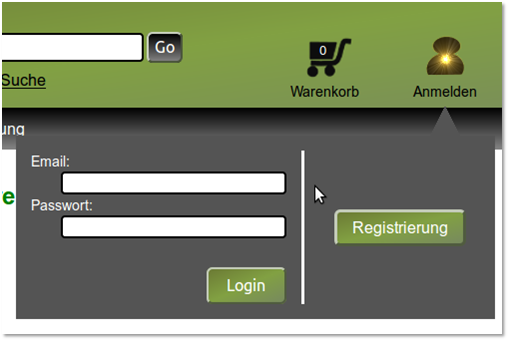
\includegraphics[width=75mm]{Bilder/Abbildung14_Loginbereich.png}
	\end{center}
	\caption{Flyout: Loginbereich}
\end{figure}

Die Besonderheit bei den Flyout des Webshops ist, dass es auch bei deaktivierten JavaScript funktioniert.  Das Flyout wurde mit den in CSS 2.0 eingeführten \glqq Kindselektor\grqq{} umgesetzt. Mit diesen \glqq Kindselektor\grqq{} ist es eingeschränlt möglich mit CSS eventbasiert zu programmieren. Um diese CSS-Funktion nutzen zu können, muss aber folgende Bedingung erfüllt sein: Das Fenster, dass angezeigt werden soll muss ein Kindelement des Elements sein, welches das Ereignis auslöst. Die Syntax des \glqq Kindselektors\grqq{} sieht wie im \textit{Quellcode 3} zeigt aus. Am Anfang steht die Bedingung, die am Elternelement erfüllt sein muss. Beim Webshop wäre es die Bedingung, dass die Maus sich auf den Anmeldesymbol befinden soll. Diese Bedingung sieht in CSS geschrieben folgendermaßen aus: \glqq .accountCell:hover\grqq{}. Darauf folgt ein \glqq >\grqq{}-Zeichen. Dieses Zeichen legt fest, dass bei erfüllter Bedingung nicht die Style-Anweisung des Elternelements verändert werden soll, sondern die Style-Anweisung eines Kindelementes. Nachfolgend wird das Kindelement angegeben, wo die Style-Anweisung geändert werden soll. Der letzte Teil der Style-Anweisung legt das neue Aussehen des Kindelements fest. Beim Webshop wird hier festgelegt, dass das Kindelement sichtbar werden soll. Ein Paar Zeilen vorher definiert eine Anweisung, dass das Kindelement unsichtbar sein soll. Bei gültiger Bedingung wird diese Anweisung wird einfach von der eben genannten Anweisung überschrieben.

\begin{center}
	\begin{lstinputlisting}[language=CSS, caption={Loginbereich: Umsetzung des Flyouts mit CSS 2.0}]
		{Quellcode/flylayout.css}
	\end{lstinputlisting}
\end{center}

\textbf{Kundenprofil ändern}\\
Hat sich eine Kunde angemeldet, so bietet der Webshop ihn die Möglichkeit die bestehenden Login-Daten und die persönlich Anschrift zu ändern. Erreicht können die Formulare zur Änderung der Daten über ein Flyout. Wenn der Kunde angemeldet ist wird das Flyout unter den Anmeldesymbol zu einen Menü geändert (siehe \textit{Abbildung 17}).
\begin{figure}[H]
	\begin{center}
			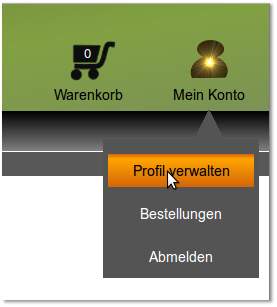
\includegraphics[width=55mm]{Bilder/Abbildung15_Menue_Profil_aendern.png}
	\end{center}
	\caption{Flyout: Kunde angemeldet}
\end{figure}

Bei diesem Menü muss der Eintrag \glqq Profil verwalten\grqq{} gewählt werden, um die bestehenden Login-Daten und die persönlich Anschrift ändern zu können. Nach der Anwahl des Eintrags bekommt der Kunde die in der \textit{Abbildung 18} gezeigte Seite zu sehen.
\begin{figure}[H]
	\begin{center}
			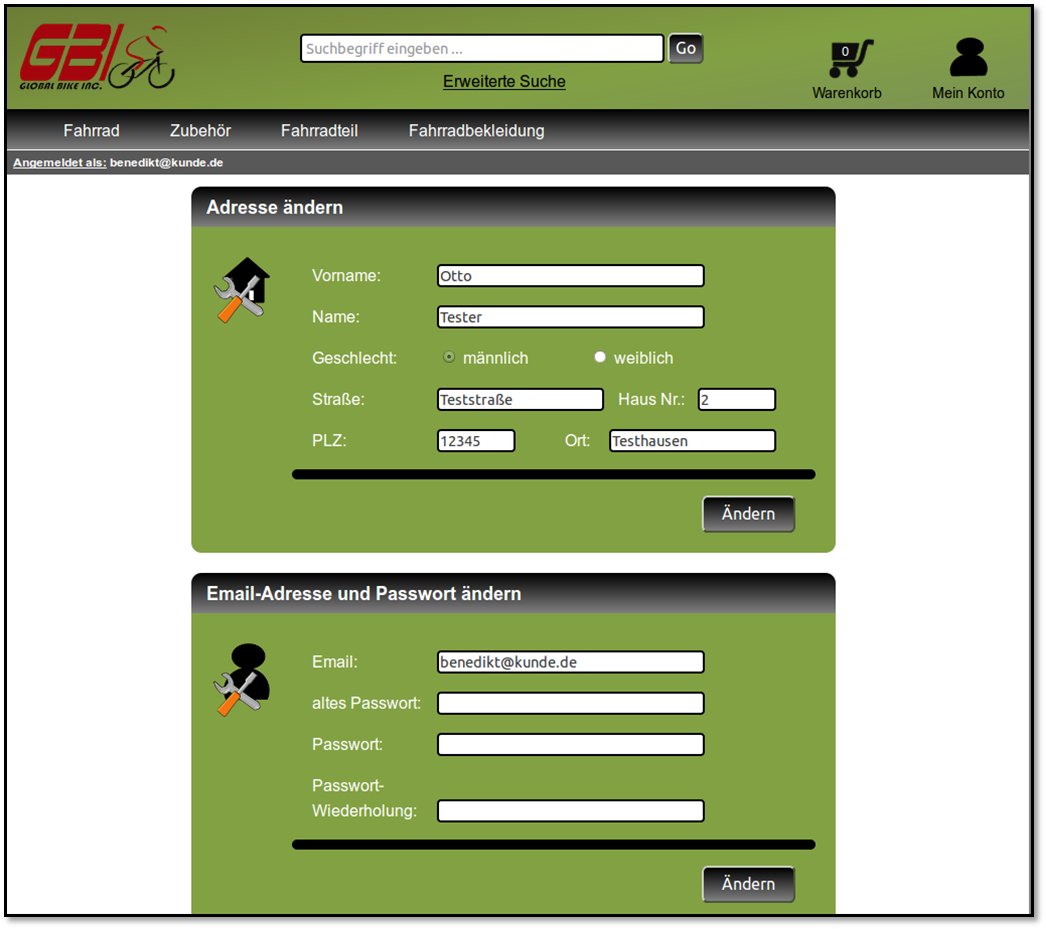
\includegraphics[width=130mm]{Bilder/formulare_profil_aendern.png}
	\end{center}
	\caption{Formulare Kundenprofil ändern}
\end{figure}
Die Änderung des Kundenprofils wurde mit Hilfe von zwei Formularen umgesetzt. Das erste Formular ändert die Anschrift des Kunden und das andere die Logindaten. Der Vorteil dieser zwei Formulare ist, dass somit die Seite übersichtlicher gestaltet ist und meist eh nur der Kunde die Adresse ändert, wenn er umgezogen ist. Häufiger wird es wahrscheinlich vorkommen, dass der Kunde das Loginpasswort ändert. Durch die Trennung der Adresse und der Logindaten werden bei Änderung des Passworts nur das neue Passwort und die Login-Email-Adresse an den Server übertragen und neu in die Datenbank geschrieben. Somit werden so wenig wie möglich unnötige Daten zum Server übertragen.\\
Technisch umgesetzt wurde der Vorgang wie beim Registrierungsvorgang. Wenn JavaScript aktiviert ist, überprüft die JavaScript-Funktion \glqq vorcheckEingabeEmailPasswort()\grqq{} oder \glqq vorcheckEingabeAdresse()\grqq{} browserseitig die Eingabe. Die aufgerufene Funktion ist abhängig von welchen Formular der Submit-Button geklickt wurde. Diese Funktionen sind in der Datei \glqq /Funktions/JS/ \\ vorcheck\_profil\_aendern.js\grqq{} vorzufinden. War die Überprüfung nicht erfolgtreich wird wieder eine Fehlermeldung auf den entsprechenden Formular ausgegeben. War die Überprüfung erfolgreich wird aus den bekannten Gründen diese nochmal auf dem Server durchgeführt. War die serverseitige Überprüfung erfolgreich, ruft die Funktionsdatei \glqq /Funktions/PHP/kunde\_aendern.php.inc\grqq{} die entsprechende Änderungsmethode der Klasse \glqq Kunde\grqq{} auf und übergibt der Methode als Parameter die Formulareingabe. Diese Methode ändert die entsprechenden Werte in der Datenbank mit Hilfe einer Update-SQL-Anweisung. Wurde die Änderung erfolgreich ausgeführt, wird der Kunde über eine Informationsbox darüber informiert.

\subsubsection{Arbeitspaket 7: Entwickeln einer Suchfunktion}